% Chapter 2

\chapter{Présentation de l'IRMA} % 2 nd chapter title

\label{Chapter2} % For referencing the chapter elsewhere, use \ref{Chapter2} 

\textit{Les informations présentées dans cette section sont entièrement issues du \href{http://irma.math.unistra.fr/}{site web de l'IRMA}}.

Créée en 1966 par Jean \textsc{Frenjel} et Gearges \textsc{Reeeb}, l'IRMA\footnote{Institut de Recherche Mathématique Avancée} est une unité mixte de recherche (UMR 7501) sous la double tutelle du CNRS (à travers l'INSMI\footnote{Institut National des Sciences Mathématiques et de leurs Interactions}) et de l’Université de Strasbourg (à travers l'UFR de Mathématique et d’Informatique).

Dirigée par le professeur Philippe \textsc{Helluy}, l'IRMA comporte environ 130 membres. On y compte environ 87 chercheurs et enseignants-chercheurs permanents et une quarantaine de membres non permanents repartis en 7 équipes de recherche.

Les activités majeures de l'entreprise sont l'organisation des séminaires, des journées, des colloques et des conférences. Ces activités sont renforcées par les nombreux partenariats qu'elle maintient dans les secteurs académique (Cemosis, Labex IRMIA, etc.) et indutriel (AxesSIM, Electis, etc.).

%----------------------------------------------------------------------------------------

\section{Structure}
L'organigramme de l'entreprise est représenté à la figure \ref{fig:OrganigrammeIRMA}.

\begin{figure}[!h]
\centering
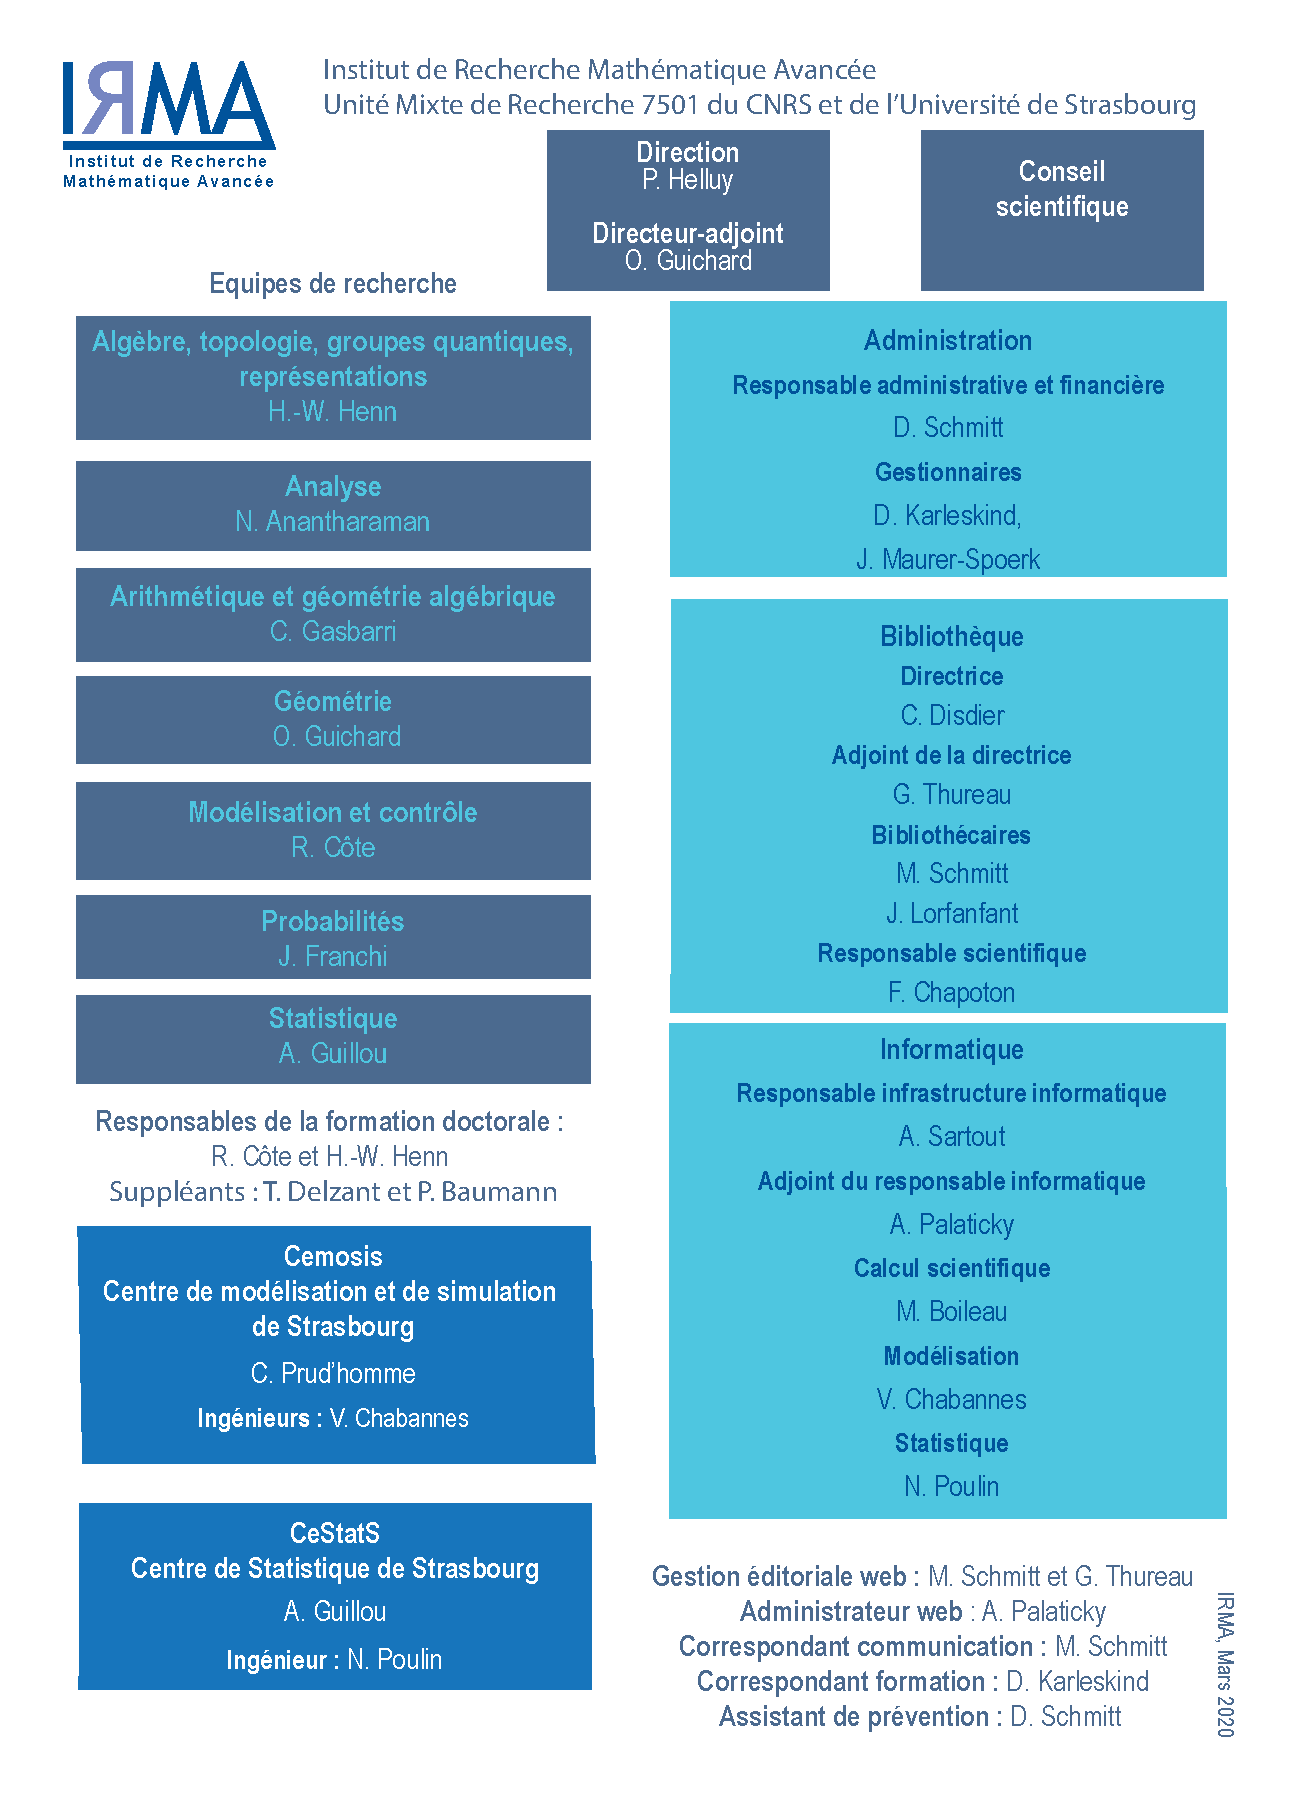
\includegraphics[width=.8\linewidth]{OrganigrammeIRMA} 
\decoRule
\caption[Organigramme de l'IRMA]{Organigramme représentant l'organisation de l'IRMA au mois de mars 2020 \parencite{Reference7}}
\label{fig:OrganigrammeIRMA}
\end{figure}

%----------------------------------------------------------------------------------------

\section{Les équipes}

L'équipe MOCO \footnote{MOdélisation et COntrôle} se compose de spécialistes des EDP, de la théorie du contrôle, du calcul scientifique, du calcul haute performance et des statistiques. Les enseignants-chercheurs MM. Emmanuel \textsc{Franck} et en Laurent \textsc{Navoret} y sont responsables des séminaires en équations aux dérivées partielles (EDP). 

L'équipe Probabilités est composée d'experts en statistique et calcul de probabilité. Ses membres se retrouvent régulièrement lors du Séminaire Stochastique. C'est à cette équipe qu'appartient M. Vincent \textsc{Vigon}. 

Je tiens une fois de plus à remercier les trois chercheurs mentionnés ci-hauts qui ont encadré ce stage. La combinaison des deux équipes dont ils font partie a permis de faire face aux deux aspects de ce stage ; premièrement la simulation d'EDP et deuxièmement l'utilisation des réseaux de neurones.

%----------------------------------------------------------------------------------------
